\documentclass[reprint, english,notitlepage]{revtex4-1}  % defines the basic parameters of the document
% if you want a single-column, remove reprint

% allows special characters (including æøå)
\usepackage[utf8]{inputenc}
\usepackage [norsk]{babel} %if you write norwegian
%\usepackage[english]{babel}  %if you write english


%% note that you may need to download some of these packages manually, it depends on your setup.
%% I recommend downloading TeXMaker, because it includes a large library of the most common packages.

\usepackage{physics,amssymb}  % mathematical symbols (physics imports amsmath)
\usepackage{graphicx}         % include graphics such as plots
\usepackage{xcolor}           % set colors
\usepackage{hyperref}         % automagic cross-referencing (this is GODLIKE)
\usepackage{tikz}             % draw figures manually
\usepackage{listings}         % display code
\usepackage{subfigure}        % imports a lot of cool and useful figure commands
\usepackage{verbatim}
\usepackage{adjustbox}

\newcommand\numberthis{\addtocounter{equation}{1}\tag{\theequation}}

% defines the color of hyperref objects
% Blending two colors:  blue!80!black  =  80% blue and 20% black
\hypersetup{ % this is just my personal choice, feel free to change things
    colorlinks,
    linkcolor={red!50!black},
    citecolor={blue!50!black},
    urlcolor={blue!80!black}}

%% Defines the style of the programming listing
%% This is actually my personal template, go ahead and change stuff if you want
\lstset{ %
	inputpath=,
	backgroundcolor=\color{white!88!black},
	basicstyle={\ttfamily\scriptsize},
	commentstyle=\color{magenta},
	language=Python,
	morekeywords={True,False},
	tabsize=4,
	stringstyle=\color{green!55!black},
	frame=single,
	keywordstyle=\color{blue},
	showstringspaces=false,
	columns=fullflexible,
	keepspaces=true}

\begin{document}



\title{Lab 2 - Strøm og spenning}
\date{\today}
\author{Candidate 073402}
\affiliation{FYS2150, Universitetet i Oslo}


\newpage

\begin{abstract}
Jeg har studert lys som er observert fra en fjern stjerne på ti forskjellige dager over en toukers periode. Ved å se på Doppler-forskyvning av en spektrallinje har jeg klart å beregne stjernens hastighet i forhold til oss ved hver av de ti målingene. På bakgrunn av dette kunne jeg slå fast at stjernen beveger seg bort fra oss med en gjennomsnittshastighet på ca. 15km/s. Den beveger seg i tillegg i bane med svært kort omløpsperiode, bare rundt 10 dager, og høy banefart, ca. 1.5km/s. Dette indikerer tilstedeværelsen av et annet massivt legeme like i nærheten.

For å finne eksakte verdier for bølgelengden til absorpsjonslinjen i det Doppler-forskjøvede spekteret brukte jeg minste kvadraters metode. Termiske bevegelser i gassene på stjernens overflate, og annen støy, gjør at dette kan være vanskelig å gjøre med øyemål. Jeg har anvendt modeller for fluks og støy som bygger på normalfordelingen, noe som har vist seg å være fornuftige antakelser.
\end{abstract}
\maketitle                                % creates the title, author, date & abstract



\section{Introduksjon}

Måling av støm, spenning og motstand er svært sentralt i eksperimentell fysikk, ikke bare fordi kunnskap om disse størrelsene og måling av dem er viktige i seg selv, men også fordi instrumenter vi bruker til å måle mange andre størrelser ofte gir elektriske signaler som vi må tolke. Dette gjelder både i vitenskapelige eksperimenter og i industrielle og praktiske anvendelser, eksempelvis temperatur og trykk.

Vi har i dette eksperimentet sett på egenskapene til multimetre som kan brukes til å måle både spenning, strøm og motstand. Vi har sett på forskjellen mellom å bruke multimetrene til å måle motstand direkte og i stedet måle strøm og spenning for siden å bruke Ohms lov til å beregne motstanden i kretsen. Til sist har vi brukt både multimetre og et oscilloskop til å studere elektrisk signal som er laget av en signalgenerator og brukt de samme redskapene til å se på forskjellige egenskaper ved en RC-krets.


\section{Teori}

Ohms lov, som gjelder for motstandene vi her bruker??, sier at spenningsfallet $U$ over en komponent er lik produktet av strømmen $I$ gjennom komponenten og resistansen $R$ til komponenten:
\begin{equation}
  \label{eq:ohms_lov}
  U = R I
\end{equation}



\section{Eksperimentelt}

Sidene multimeterne Fluke 45 og Fluke 75 er brukt gjennom hele forsøket vil jeg begynne med å angi måleusikkerheten til disse. BLABLABLA

\subsection{Multimeter måler multimeter}
Her har vi brukt de to multimeterne, Fluke 45 og Fluke 75, og latt dem måle på hverandre. På den måten har vi målt motstanden til hvert av multimetrene i Voltmeter- og Amperemeterfunksjon, strømmen gjennom dem i Voltmeter- og Ohmmeterfunksjon og spenningen over dem i Amperemeter- og Ohmmeterfunksjon. Kretstegninger er vist i figur \ref{fig:krets_multi_maaler_multi}.
\begin{figure}
  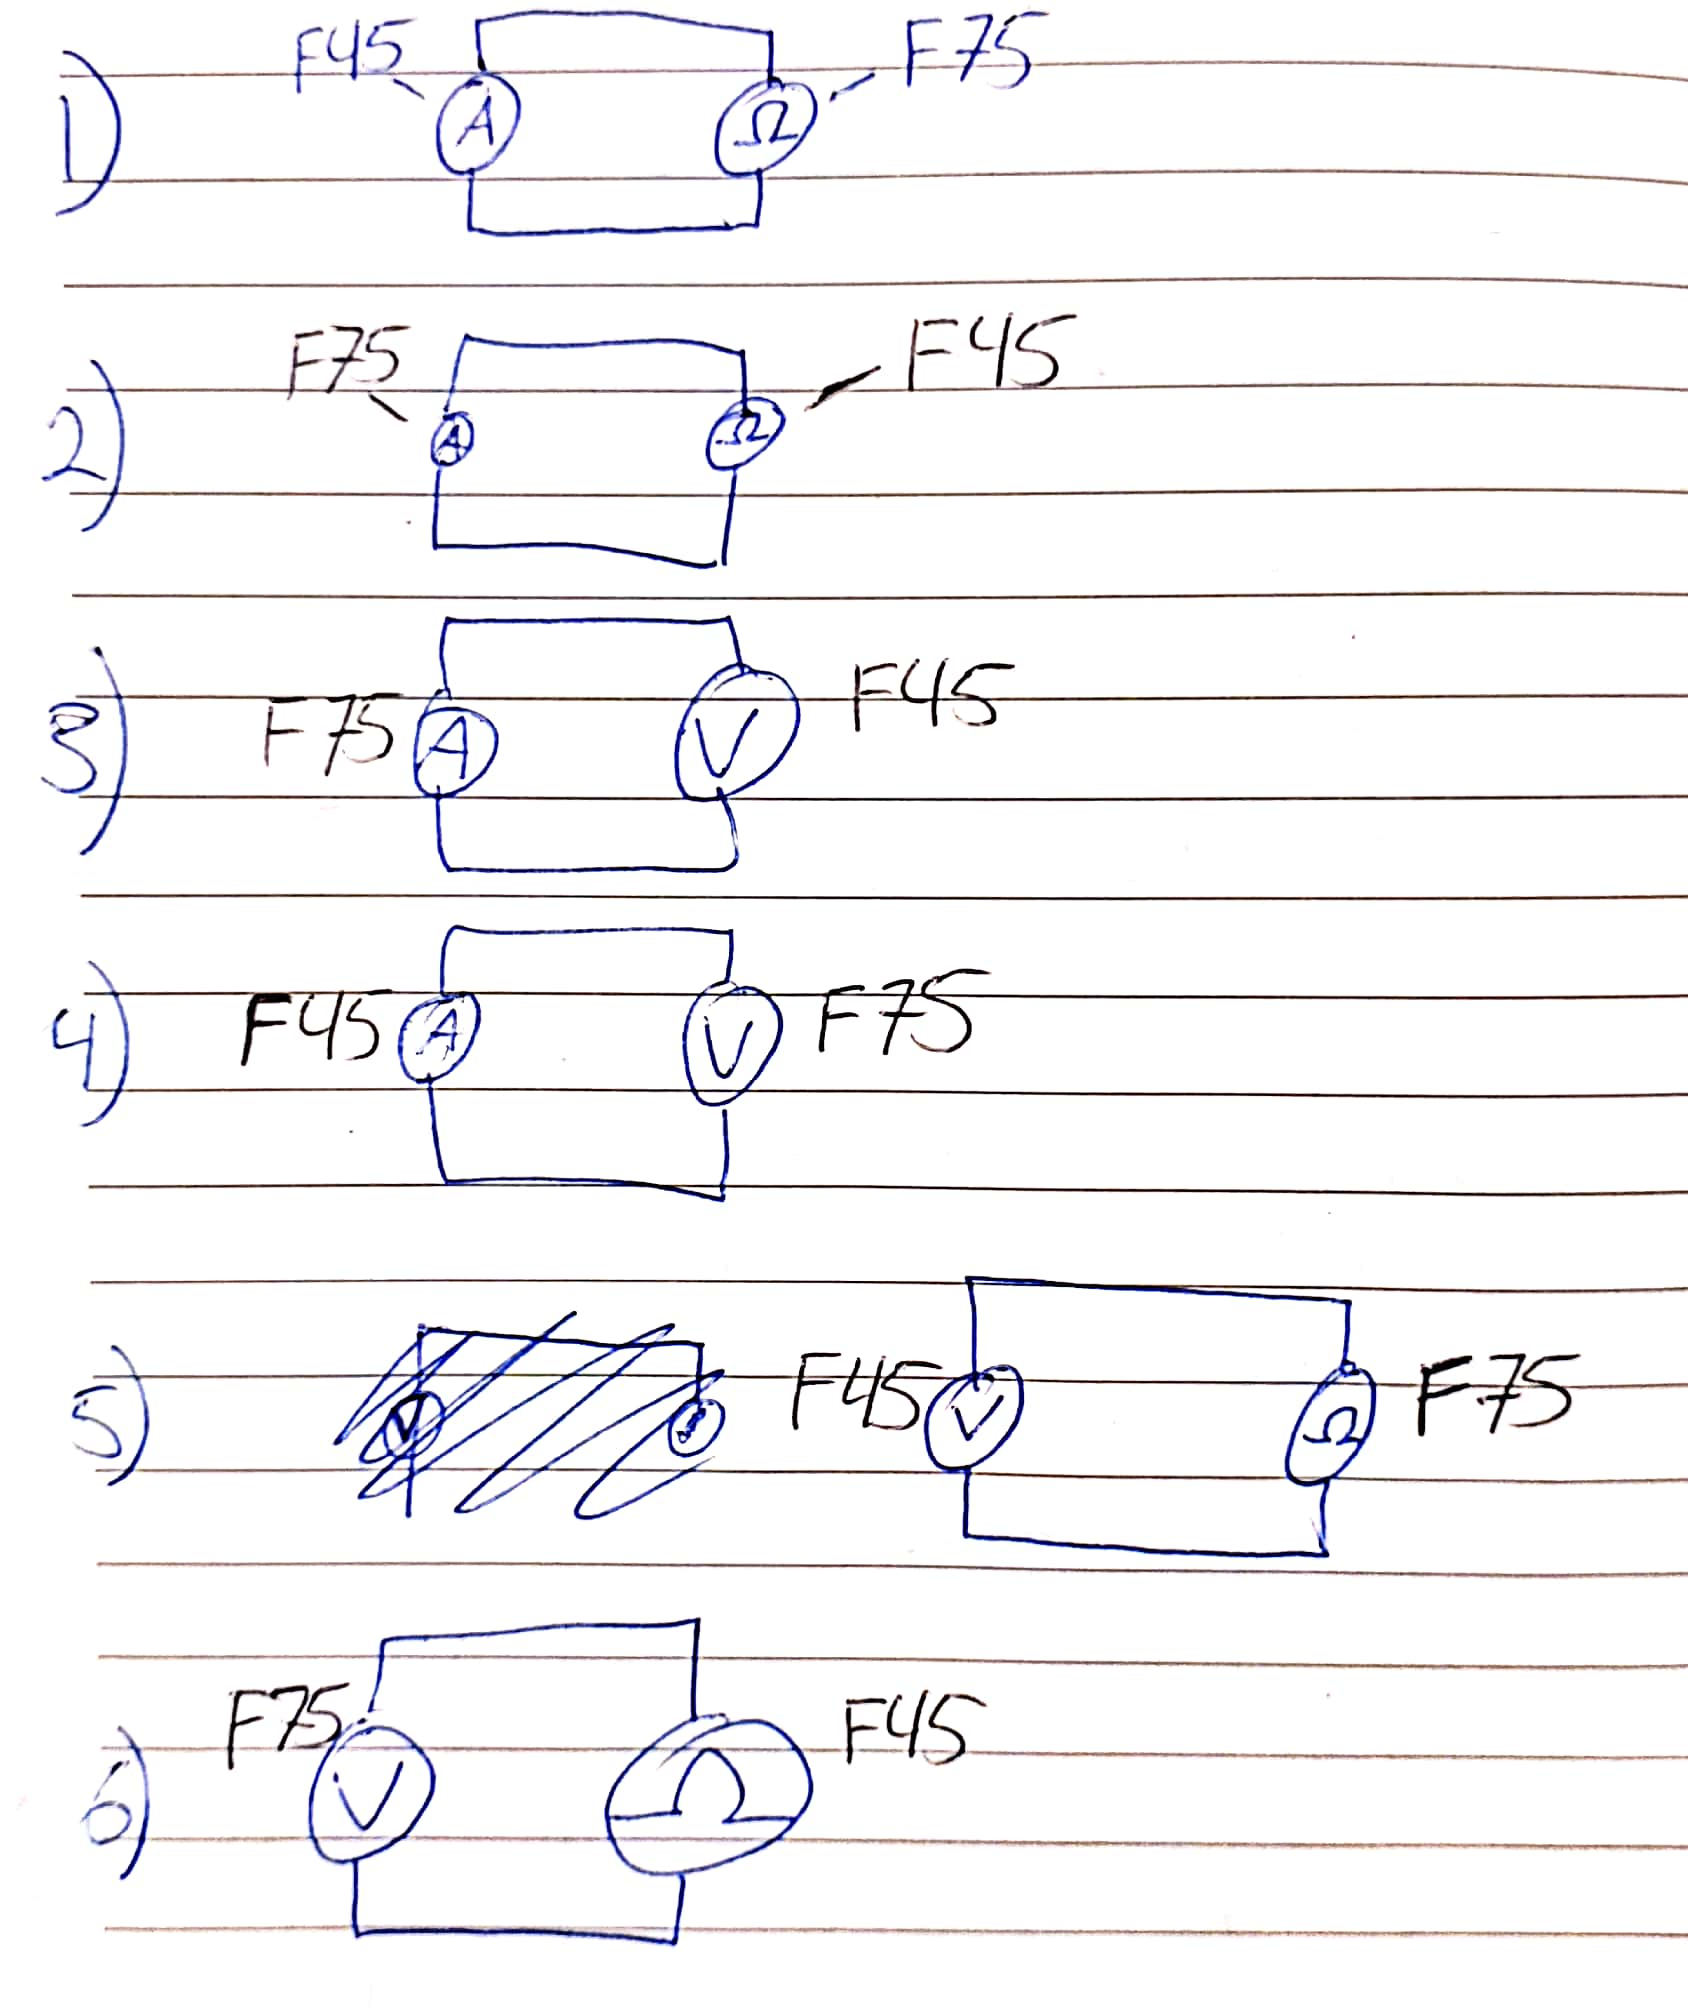
\includegraphics[width=\linewidth]{krets_multi_maaler_multi.jpg}
  \caption{Kretstegninger som viser hvordan vi har koblet i de forskjellige målingene der multimeterne måler på hverandre. F45 og F75 viser til henholdsvis Fluke 45 og Fluke 75.}
  \label{fig:krets_multi_maaler_multi}
\end{figure}

Deretter skal vi studere kretstegningene i figur \ref{fig:krets_ulike_funksjoner_multimeter} som viser et Amperemeter, et Voltmeter og et Ohmmeter. Oppgaven er å avgjøre hvilken kretstegning som svarer til hvilken funksjon.
\begin{figure}
  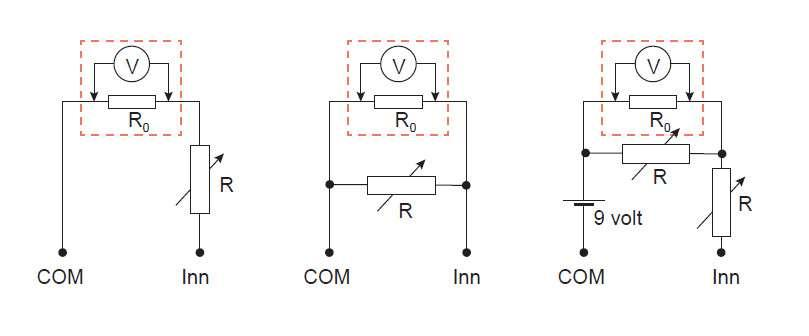
\includegraphics[width=\linewidth]{krets_ulike_funksjoner_multimeter.jpeg}
  \caption{Kretstegning for de tre ulike funksjonene til et multimeter (Amperemeter, Voltmeter og Ohmmeter). Oppgaven er å avgjøre hvilken kretstegning som svarer til hvilken funksjon. Motstandene $R$ med pil gjennom har variabel resistans, mens $R_0$ er uendret.}
  \label{fig:krets_ulike_funksjoner_multimeter}
\end{figure}


\subsection{Motstand, likestrøm og likespenningsmålinger med multimeter}
Her skal vi måle resistansen til to motstander, først direkte med Fluke 45 i Ohmmeterfunksjon og siden ved å bruke begge multimeterne til å måle strøm og spenning i en krets. Dersom vi kjenner strøm og spenning i kretsen kan vi bruke Ohms lov \ref{eq:ohms_lov} til å beregne motstanden i kretsen. Målepunktene vi bruker for spenning og strøm er vist i kretstegningen i figur \ref{fig:krets_motstander}. Siden vi bare har to multimetre, må vi koble om for å måle alle tre størrelser $V_{\text{inn}}$, $V_{\text{ut}}$ og $I$.
\begin{figure}
  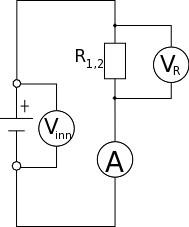
\includegraphics[width=\linewidth]{krets_motstander.jpg}
  \caption{Kretstegning som viser hvordan vi måler strøm og spenning når vi skal bestemme motstandene R1 og R2 ved hjelp av Ohms lov. Vi brukte Fluke 45 til å måle strømmen og Fluke 75 til å måle de to spenningene.}
  \label{fig:krets_motstander}
\end{figure}

Ohms lov (\ref{eq:ohms_lov} løst for motstand $R$ kan skrives på formen $R = U/I = U I^{-1}$. Usikkerheten i R er da gitt ved
\begin{align*}
  \Delta R &= R \sqrt{\left( \frac{\Delta U}{U} \right) ^2 + \left( -1 \frac{\Delta I}{I} \right) ^2} \\
  &= R \sqrt{\left( \frac{\Delta U}{U} \right) ^2 + \left( \frac{\Delta I}{I} \right) ^2}, \numberthis \label{eq:usikkerhet_R}
\end{align*}
der $R$ er den beregnede resistansen og $\Delta U$ og $\Delta I$ er måleusikkerhetene i spenning $U$ og strøm $I$.


\subsection{Vekselspenninger med frekvensgenerator, oscilloskop og multimeter}
Her skal vi lage etter tur to varierende spenningssignaler med en signalgenerator. Vi skal bruke et oscilloskop og et multimeter til å måle spenningen fra signalgeneratoren. De to signalene vi brukte i analysen var et sinus- og et firkantsignal. Bilder av signalene med innstillingene som ble brukt finnes i figur \ref{fig:inputsignaler}.

\begin{figure}
  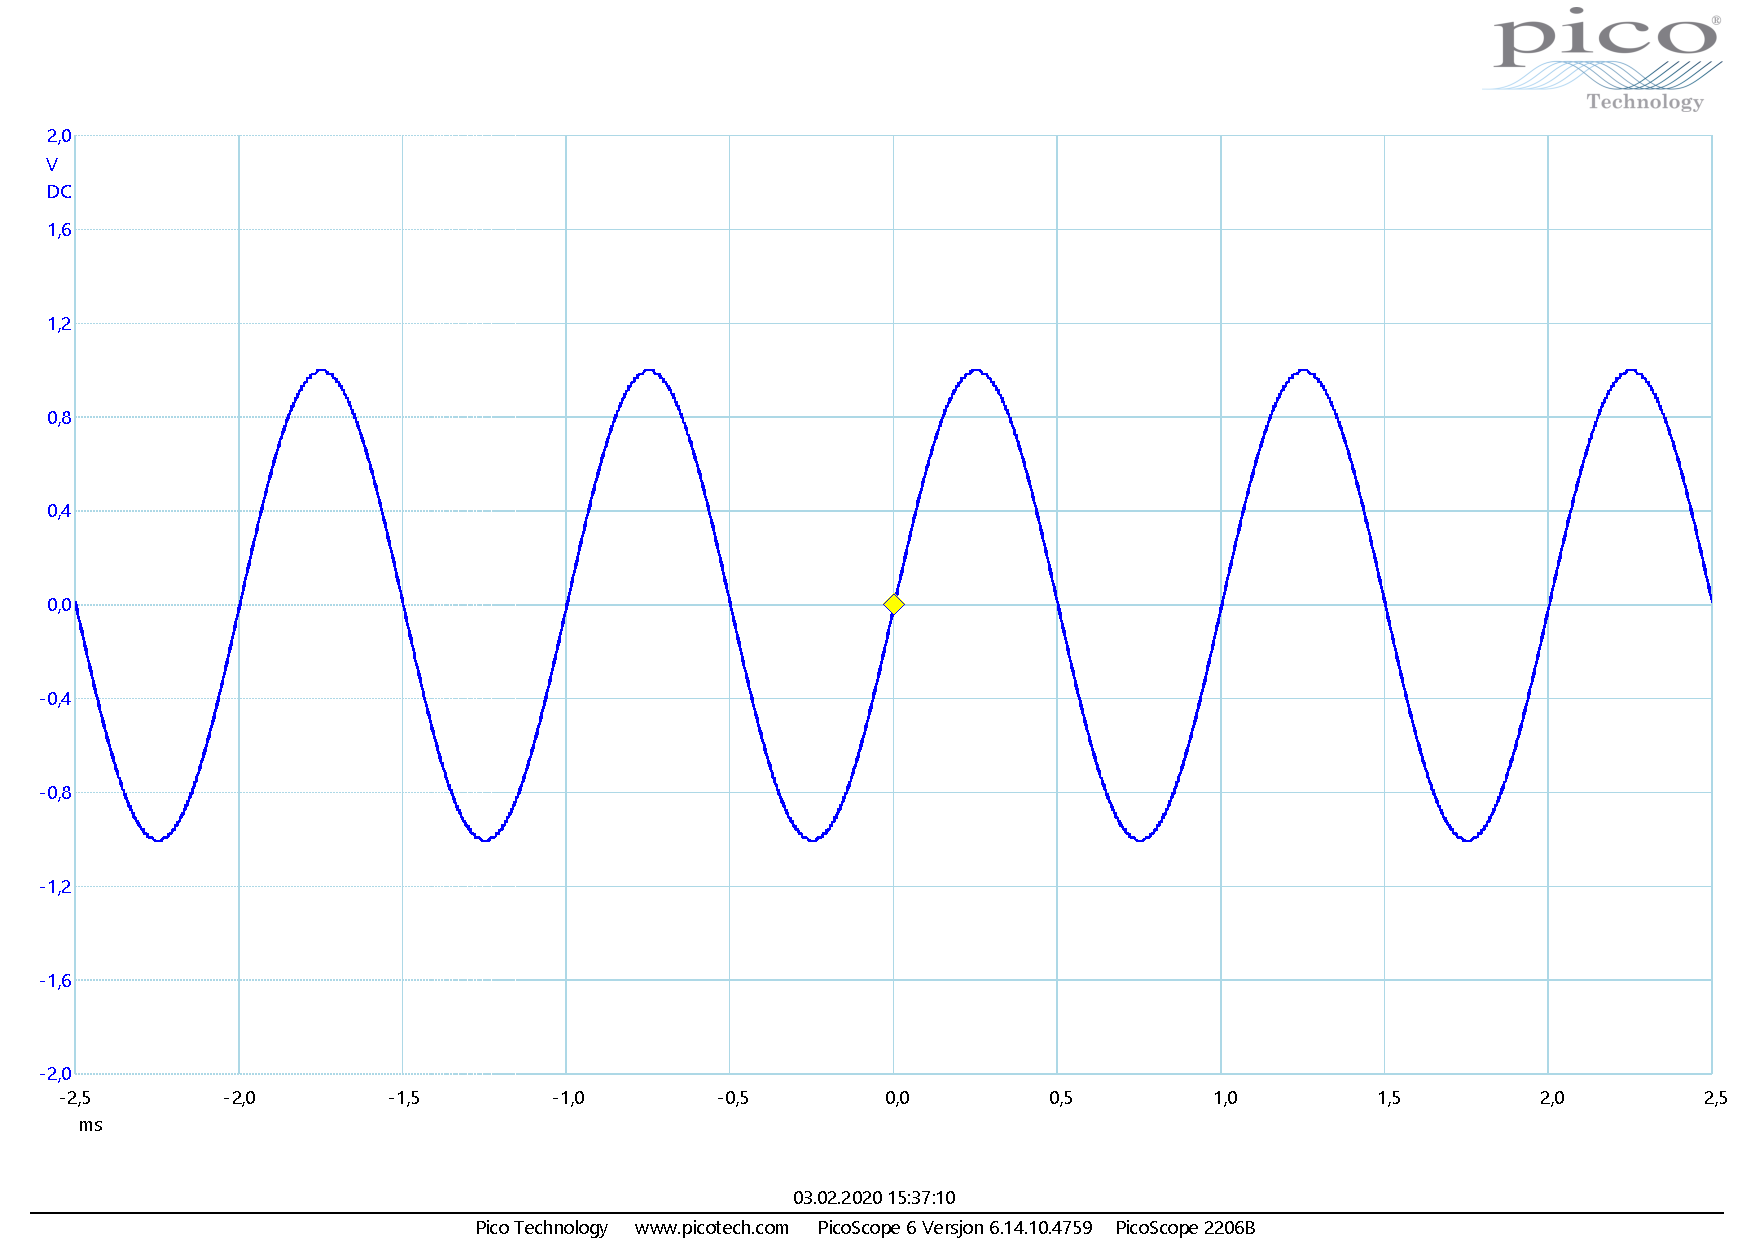
\includegraphics[width=\linewidth]{../sinus.pdf}
  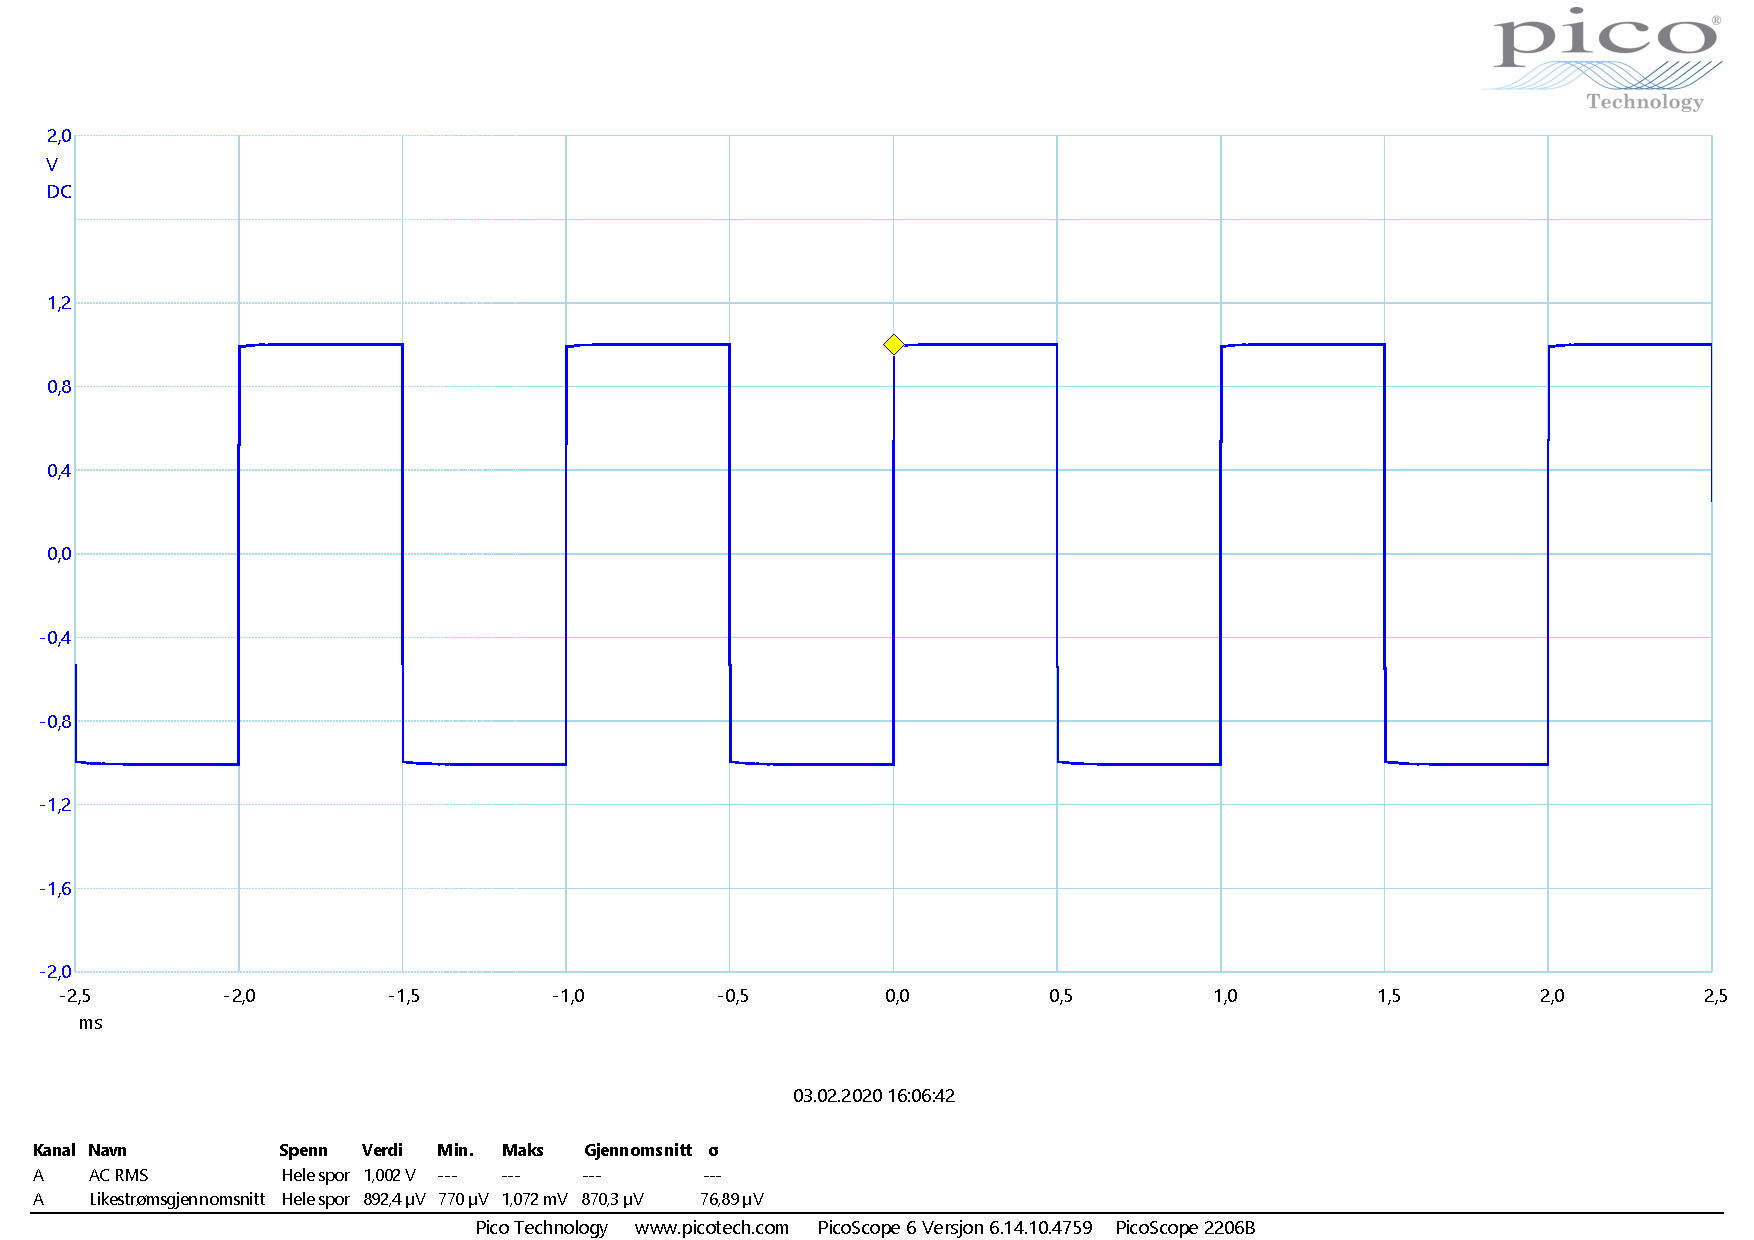
\includegraphics[width=\linewidth]{../firkant.pdf}
  \caption{Sinus- og firkantsignalet brukt til å måle vekselspenning med oscilloskop. Begge siganelene hadde en frekvens på 1 kHz og amplitude 1 V. Resten av innstillingene 500 $\mu$s/div, 1 MS, $\pm$ 2 V, AC, 12 bit.???}
  \label{fig:inputsignaler}
\end{figure}


\subsection{Krets med frekvensavhengig respons}
Vi har koblet opp en RC-krets som vist i figur \ref{fig:krets_RC}. Denne vil fungere som et lavpassfilter som filtrerer bort signaler med høye frekvenser mens den lar signaler med lavere frekvenser passere CITE?. For høye frekvenser (tilnærmingen blir bedre og bedre for høyere frekvenser) vil følgende relasjon gjelde mellom forholdet mellom spenning ut og spenning inn og frekvens:
\begin{equation}
  \log \left( \frac{V_{\text{ut}}}{V_{\text{inn}}} \right) = \log (\omega) + \log (\omega_0) \label{eq:lavpass}
\end{equation}
\begin{equation}
  \omega_0 = \frac{1}{RC} \label{eq:omega_0}
\end{equation}
Her er $\omega = 2 \pi f$, der $f$ er signalfrekvensen, mens $V_{\text{ut}}$ og $V_{\text{inn}}$ er størrelsene som er markert på figur \ref{fig:krets_RC}. $C$ er kapasitansen til kondensatoren og $R$ er resistansen til motstanden.
\begin{figure}
  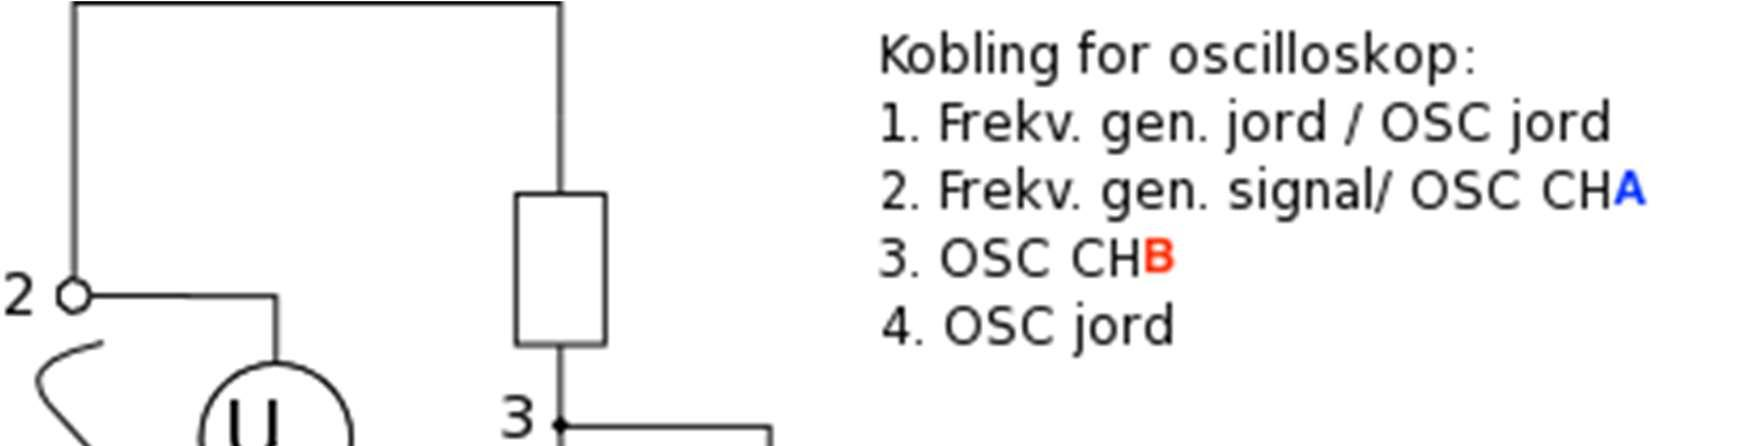
\includegraphics[width=\linewidth]{krets_RC.jpg}
  \caption{Kretstegning som viser hvordan vi kobler RC-kretsen. Motstanden R er 10 000 $\pm 150 \omega$ (usikkerheten er hentet fra datablad for motstanden).}
  \label{fig:krets_RC}
\end{figure}


Likning \ref{eq:omega_0} gir at kapasitansen er gitt ved
\begin{equation}
  \label{eq:kapasitans}
  C = \frac{1}{R \omega_0}.
\end{equation}
Dette kan skrives $C = R^{-1} \omega_0^{-1}$ som gir at usikkerheten i kapasitansen kan uttrykkes
\begin{align*}
  \Delta C &= C \sqrt{\left( -1 \frac{\Delta R}{R} \right) ^2 + \left( -1 \frac{\Delta \omega_0}{\omega_0} \right) ^2} \\
  &= C \sqrt{\left( \frac{\Delta R}{R} \right) ^2 + \left( \frac{\Delta \omega_0}{\omega_0} \right) ^2}, \numberthis \label{eq:usikkerhet_C}
\end{align*}
hvor $C$ er den beregnede kapasitansen og $\Delta R$ og $\Delta \omega_0$ er måleusikkerhetene i resistans $R$ og konstanten $\omega_0$.


\section{Resultater}

\subsection{Multimeter måler multimeter}
Den første delen av eksperimentet, å bruke hvert av multimetrene til å måle på det andre, ga resultatene presentert i tabell \ref{table:multimetre}.

\begin{table}[p]
\label{table:multimetre}
\caption{Tabell som viser resultatene av å bruke de to multimeterne til å måle på hverandre. Målingene merket med * var oppgitt med én desimal mer på måleinstrumentet enn det som er oppgitt her, men det siste sifferet er sløyfet fordi det var umulig å avlese da verdien svingte hele tiden. OL står for overload og viser at størrelsen vi prøver å måle er for stor til å vises med denne oppløsningen.}

\begin{adjustbox}{width=\linewidth}
\begin{tabular}{||c || c | c | c||}
\hline
Forsøk \# & Spenning, [mV] & Strøm, [mA] & Motstand  \\ \hline\hline
1 &            & F45: 0.501 & F75: 10.9 $\Omega$    \\ \hline
2 &            & F75: 0.81  & F45: 5.94 $\Omega$    \\ \hline
3 & F45: 0.01  & F75: 0.00  &                       \\ \hline
4 & F75: 0.0   & F45: 0.000 &                       \\ \hline
5 & F45: 722.4 &            & F75: 10.03 M$\Omega$  \\ \hline
  &     1982.2 &            &        OL. $\Omega$   \\ \hline
  &     1979.3 &            &        OL $\Omega$    \\ \hline
  &     1426.4 &            &        O.L k$\Omega$  \\ \hline
  &     1310.0 &            &        OL. k$\Omega$  \\ \hline
  &      722.3 &            &        .OL  M$\Omega$ \\ \hline
6 & F75:  1552 &            & F45: 11.10 M$\Omega$*  \\ \hline
  &       1552 &            & 11.1 M$\Omega$*        \\ \hline
  &       1552 &            & 11.1 M$\Omega$         \\ \hline
\end{tabular}
\end{adjustbox}
\end{table}

Den første kretsen i figur \ref{fig:krets_ulike_funksjoner_multimeter} svarer til Voltmeter-funksjonen. Den andre svarer til et Amperemeter, og den tredje er et Ohmmeter.


\subsection{Motstand, likestrøm og likespenningsmålinger med multimeter}
Ved å måle motstandene R1 og R2 direkte fikk vi disse verdiene:
\begin{itemize}
  \item R1 = 10.10 $\pm$ 0.01 $\Omega$
  \item R2 = 0.99 $\pm$ 0.02 M$\Omega$
\end{itemize}

Ved indirekte måling av motstanden ved Ohms lov fikk vi først verdiene for strøm og spenning som er vist i tabell \ref{table:motstander}. Ved likninger \ref{eq:ohms_lov} og \ref{eq:usikkerhet_R} fikk vi da disse verdiene for størrelsene på motstandene:
\begin{itemize}
  \item R1 = 10.37 $\pm 0.06 \Omega$
  \item R2 = 0.90 $\pm$ 0.07 M$\Omega$
\end{itemize}

\begin{table}[p]
\label{table:motstander}
\caption{Tabell som viser resultatene av å bruke de to multimeterne til å måle strøm og spenning gjennom kretsene i figur \ref{fig:krets_motstander}. Målingen merket med * er avlest for tidlig i forhold til den tiden som multimeter bruker på å stabilisere seg når man måler strøm med største presisjon, og er ikke egnet til å brukes i videre beregninger.}

\begin{adjustbox}{width=\linewidth}
\begin{tabular}{||c || c | c | c||}
\hline
Komponent & Måling & Spenning, [V] & Strøm, [mA]   \\ \hline\hline
R1 & Spenning inn     & 1.474 $\pm$ 0.007 & 68.93 $\pm$ 0.04*   \\ \hline
   & Spenning over R1 & 0.716 $\pm$ 0.004 & 69.01 $\pm$ 0.04    \\ \hline
R2 & Spenning inn     & 17.78 $\pm$ 0.08  & 0.018 $\pm$ 0.002   \\ \hline
   & Spenning over R2 & 17.79 $\pm$ 0.08  & 0.020 $\pm$ 0.002   \\ \hline
\end{tabular}
\end{adjustbox}
\end{table}


\subsection{Vekselspenninger med frekvensgenerator, oscilloskop og multimeter}
Resultatene fra målingene på det genererte signalet finnes i tabell \ref{table:AC_RMS}.
\begin{table}[p]
\label{table:AC_RMS}
\caption{Tabell som viser resultatene av å bruke oscilloskop og multimeter (Fluke 45) til å måle på sinussignal og firkantsignal laget av en signalgenerator.}

\begin{adjustbox}{width=\linewidth}
\begin{tabular}{||c || c | c | c||}
\hline
Apparat     & Sinussignal, & Sinussignal med forskyvning 1V, & Firkantsignal, \\
            & AC RMS      & likestrømsgjennomsnitt          & AC RMS        \\ \hline\hline
Oscilloskop & 707.1 mV $\pm 20 \mu$V  & 996.7 mV            & 1.002 V $\pm 50 \mu$V \\ \hline
Multimeter  & 704.75 mV   & 996.13 mV                       & 996.75 mV     \\ \hline
Analytisk   & 707.1 mV    & 1 V                             & 1V            \\ \hline
\end{tabular}
\end{adjustbox}
\end{table}

\subsection{Krets med frekvensavhengig respons}
Jeg har brukt måledataene fra filen LavpassRC\_sorted.mat, målt av foreleser og veiledere. Dataene er presentert i figur \ref{fig:LavpassRC}.
\begin{figure}
  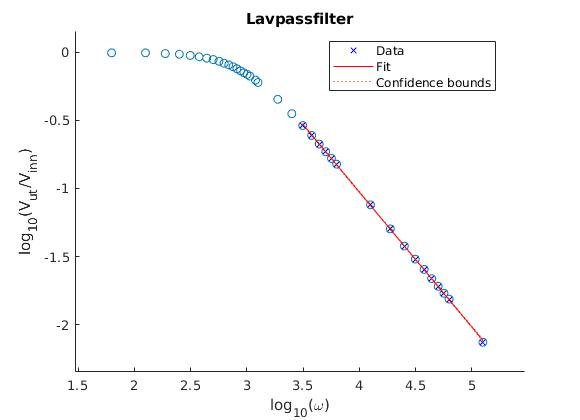
\includegraphics[width=\linewidth]{../RC_fitlm_LavpassRC_sorted.jpg}
  \caption{Datapunktene (blått) for måling av spenning og frekvens i RC-kretsen \ref{fig:krets_RC}. Lineær regresjon (rød linje) på datapunktene som svarer til de høyeste frekvensene. Den lineære tilnærmingen (som gjelder for høye frekvenser) gir at stigningstallet for den røde linja skal bli -1. Tilpasningen her gir stigningstall -0.98879 med en standardfeil på 0.0026743.}
  \label{fig:LavpassRC}
\end{figure}
Ved lineær regresjon fant jeg at verdien for $log_{10}(\omega_0)$ var 2.93 med en standard error på 0.01 som jeg bruker videre som usikkerheten i målingen. Ved likninger \ref{eq:kapasitans} og \ref{eq:usikkerhet_C} gir dette en kapasitans på $C = 1.18 \cdot 10^{-7} \pm 4 \cdot 10^{-9}$ F, der jeg har brukt at usikkerheten i R er $\Delta R =  150 \Omega$.


\section{Diskusjon}

\subsection{Multimeter måler multimeter}

I figur \ref{fig:krets_ulike_funksjoner_multimeter} viser den første kretsen et enkelt Voltmeter. Kretsen er koblet i parallell og vi ønsker å bestemme spenningsfallet $V_0$ mellom Inn og COM. Strømmen sendes gjennom kretsen og ved å måle spenningsfallet $V$ over $R_0$ kan man bestemme $V_0$:
\begin{align*}
  I = \frac{V_0}{R_0 + R} = \frac{V}{R_0}
  V_0 = V \frac{R_0 + R}{R_0}
\end{align*}
Følsomheten for $V$ er gitt, men ved å øke verdien for $R$ kan vi måle større og større spenninger.

Den andre kretsen i figuren viser et enkelt Amperemeter. Vi kan velge en liten $R$, slik at spenningsfallet over apparatet blir lite, og når vi kjenner resistansen til begge motstandene kan vi finne strømmen ved:
\begin{align*}
  I = \frac{V}{R} + \frac{V}{R_0}
\end{align*}
Ved å endre R kan man endre følsomheten til apparatet og tilpasse det ønskede måleområder.

Den tredje kretsen i figuren svarer til et Ohmmeter. Her settes det på en spenning, og resten av kretsen fungerer som et kombinert Voltmeter og Amperemeter. På den måten finner vi strømmen gjennom kretsen samt spenningsfallet over den ukjente motstanden hvilket lar oss bestemme resistansen ved hjelp av Ohms lov.

Av tabell \ref{table:multimetre} kan man lese av typiske motstander for de forskjellige kretsene. Vi ser at motstanden gjennom multimeterne i Amperemeterfunksjon er ca 6 $\omega$ og 11 $\omega$. Vi ønsker at motstanden gjennom et Amperemeter skal være så liten som mulig for å unngå et spenningstap over måleinstrumentet. Siden resistansene ikke er null, kan apparatene ha merkbare påvirkninger på kretsen de måler på dersom resten av motstandene i kretsen ikke er store i forhold til motstanden til måleapparatet. Det virker som at Fluke 75 har mindre resistans enn Fluke 45, men Fluke 45 (som er et lab-multimeter) har høyere oppløsning.

Når vi lar et Amperemeter og et Voltmeter måle på hverandre, blir begge målingene (tilnærmet) null. Det er fordi det da ikke er noen spenningskilde i kretsen. De eneste tilfellene hvor det går strøm i kretsen er når det ene av måleapparatene er et Ohmmeter. Et Ohmmeter setter selv på en spenning på kretsen, det må det gjøre for å kunne bestemme motstanden vi prøver å måle. Amperemetre og Voltmetre kobles på i kretser der vi allerede har en ekstern spenningskilde som får det til å gå strøm i kretsen.

Av målinger 5 og 6 ser vi at motstanden til multimeterne i Voltmeter-funksjon er 10-11 M$\Omega$. Vi ønsker at motstanden gjennom et voltmeter skal være så stor som mulig, slik at ingen strøm går gjennom det når vi kobler det i parallell med kretsen vi ønsker å måle på. Her er motstanden til Fluke 75 størst, som i utgangspunktet er det vi ønsker. Vi må likevel huske på at det ikke er teoretisk mulig å lage et Amperemeter med null motstand eller et Voltmeter med uendelig motstand. Selv om dette er det vi ønsker, må vi gjøre en avveiing mellom hvor mye apparatene påvirker kretsen og hvor følsomme apparatene skal være.

Det er katastrofalt dersom man kobler et multimeter i Amperemeterfunksjon direkte på en spenningskilde fordi motstanden i Amperemeteret er veldig liten. Strømmen gjennom apparatet blir derfor stor, og effekten $P = U I$ blir stor, noe som kan skade komponentene, og kanskje også kortslutte kretsen.


\subsection{Motstand, likestrøm og likespenningsmålinger med multimeter}

Fra resultatene ser vi at vi fikk betydelig lavere usikkerhet ved å måle resistansen direkte, enn det vi gjorde ved å måle strøm og spenning for så å anvende Ohms lov. Dette er fornuftig ettersom vi ved den indirekte metoden gjør flere målinger, som hver har usikkerheter som siden kombineres. Vi ser at verdiene for R2 såvidt overlapper dersom vi tar hensyn til usikkerhetene, mens de to verdiene for R1 ikke overlapper i det hele tatt. Det er grunn til å at den indirekte målingen av R1 blir uriktig fordi resistansen i Amperemeteret ikke er neglisjerbar i forhold til resistansen i motstanden. Dette ser vi tydelig av tabell \ref{table:motstander}, der inn-spenningen er mye større enn spenningsfallet over R1. Dette kan forklares ved at vi også har et betydelig spenningsfall over Amperemeteret, og vi ser at de flere måleapparatene tydelig påvirker kretsen.


\subsection{Vekselspenninger med frekvensgenerator, oscilloskop og multimeter}

Det virker fra tabell \ref{table:AC_RMS} som at alle målinger stemmer godt overens med de teoretiske resultatene (gitt at signalene som blir generert også er riktige). Målingene fra oscilloskopet er nærmere det teoretiske i alle målinger, dette apparatet er nok det mest nøyaktige. For å måle forskyvningen kan vi bruke et Voltmeter eller funksjonen for likestrømsgjennomsnitt i oscilloskopet.


\subsection{Krets med frekvensavhengig respons}

Det er tydelig av figur \ref{fig:LavpassRC} at en logaritmisk fordeling på aksene er fornuftig for å studere dataene. For høye frekvenser er en lineær modell en svært god tilpasning, noe som viser seg i den lave standardfeilen i lineærtilpasningen og den lave usikkerheten vi til slutt får for kapasitansen.

Vi ser for øvrig tydelig at signaler med høy frekvens blir filtrert bort. Forholdet $V_{\text{ut}}/V_{\text{inn}}$ forteller oss hva styrken er på signalene som kommer ut av kretsen i forhold til styrken på signalet idet det kommer inn. Av figur \ref{fig:LavpassRC} ser vi at for lave frekvenser er dette forholdet ca. 1 ($\log (V_{\text{ut}}/V_{\text{inn}}) \approx 0$ gir $V_{\text{ut}}/V_{\text{inn}} \approx 1$) som betyr at signalstyrken blir bevart. For høye frekvenser derimot, blir signalstyrken mer og mer redusert (det viser seg i at forholdet blir mindre og mindre). Signaler med lav frekvens bevares, mens signaler med høy frekvens blir filtrert bort. 



\section{Konklusjon}
blablabla



\onecolumngrid
\vspace{1cm} % some extra space


\begin{thebibliography}{}
\bibitem[Hansen (2017)]{part1A} Hansen, F. K.,  2017, Forelesningsnotat 1A i kurset AST2000
\bibitem[Hansen (2017)]{part1C} Hansen, F. K.,  2017, Forelesningsnotat 1C i kurset AST2000
\bibitem[Hansen (2017)]{part1D} Hansen, F. K.,  2017, Forelesningsnotat 1D i kurset AST2000
\bibitem[5]{wiki} Solen, https://no.wikipedia.org/wiki/Solen, Lest 17.10.19

\end{thebibliography}

\end{document}
